\documentclass[class=report,crop=false]{standalone}
\usepackage[screen]{../exo7book}

% Commande ponctuelle
\newcommand{\alenvers}[1]{\rotatebox[origin=c]{180}{#1}}
\newcommand{\vect}{\overrightarrow}

\begin{document}

%====================================================================
\chapitre{Calcul formel}
%====================================================================

%\insertvideo{lSn_KZvTCOs}{partie 9. \'Equations différentielles}

%%%%%%%%%%%%%%%%%%%%%%%%%%%%%%%%%%%%%%%%%%%%%%%%%%%%%%%%%%%%%%%%
\setcounter{section}{8}
\section{\'Equations différentielles}


%--------------------------------------------------------
\subsection{\'Equations différentielles $y' = f(x,y)$}

La commande \codeinline{desolve} permet de résoudre formellement des équations différentielles.
Consultez la documentation, accessible par \codeinline{help(desolve)}.

\begin{tp}
\sauteligne
\begin{enumerate}
  \item 
  \begin{enumerate}
    \item Résoudre l'équation différentielle :
  $$y' = y + x + 1.$$
  Il s'agit donc de trouver toutes les fonctions $x\mapsto y(x)$ dérivables, telles que
  $y'(x) = y(x) + x + 1$, pour tout $x\in \Rr$.
    
    \item Résoudre l'équation différentielle en ajoutant une condition initiale :
  $$y' = y + x + 1 \quad \text{ et } \quad y(0)=1.$$
  \end{enumerate}
  
  

  \item 
  \begin{enumerate}
    \item
    Résoudre sur $\Rr_+^*$ l'équation différentielle :
    $$x^2y' = (x-1)y.$$ 
    \item Trouver la solution vérifiant $y(1)=2$.
    
    \item Peut-on trouver une solution sur $\Rr$ ?
  \end{enumerate}
    
  \item Calculer la \defi{fonction logistique}, solution
  de l'équation différentielle $$y'= y(1-y) - 1.$$       
\end{enumerate}
\end{tp}

\begin{enumerate}
  \item  
  
  \begin{enumerate}
  \item 
On commence par déclarer la variable $x$. 
On définit une fonction $x \mapsto y(x)$ ainsi que sa dérivée $y'(x)$ 
par \codeinline{diff(y,x)}. 
On prendra ici la convention de noter $y'$ par \codeinline{yy}.
L'équation différentielle $y' = y + x + 1$
s'écrit donc \codeinline{yy == y+x+1}.

  \insertcode{algos/equadiff-intro-tex1.sage}{equadiff-intro.sage (1)}

On lance la résolution de l'équation différentielle par un appel à la fonction  
\codeinline{desolve}, avec pour argument 
l'équation différentielle à résoudre, ainsi que la fonction inconnue, qui est ici $y$. 
\Sage\ renvoie :\\
\centerline{\codeinline{-((x + 1)*e^(-x) - _C + e^(-x))*e^x}}
où \codeinline{_C} désigne une constante arbitraire.
Après simplification évidente, les solutions sont les :
$$y(x) = -x-2 + C \exp(x) \quad \text{ où } \quad C \in \Rr.$$

    \item Il est possible de préciser une condition 
initiale grâce à l'argument optionnel \codeinline{ics} 
(voir la dernière ligne du code ci-dessus), ici on 
spécifie donc que l'on cherche la solution vérifiant $y(0)=1$.
L'unique solution est alors : $y(x) = -x-2 + 3\exp(x)$, c'est-à-dire correspondant à $C=3$.

  \end{enumerate}

  \item 
  \begin{enumerate}
    \item En se restreignant à $\Rr_+^*$ ($x>0$), on trouve $y(x) = Cx \exp(\frac1x)$, $C\in \Rr$.
\insertcode{algos/equadiff-intro-tex2.sage}{equadiff-intro.sage (2)}
    
    \item La solution vérifiant $y(1)=2$ est $y(x) = 2x \exp(\frac1x - 1)$,
    c'est-à-dire $C = 2 \exp(-\frac1e)$.
    
    \item Sur $\Rr_-^*$ ($x<0$), les solutions sont aussi de la forme $y(x) = Cx \exp(\frac1x)$.

      \insertcode{algos/equadiff-intro-tex2bis.sage}{equadiff-intro.sage (2)}
    La seule solution définie sur $\Rr$ est donc la fonction nulle $y(x) = 0$ (et $C=0$). 
    En effet, si $C \neq 0$ il n'y a pas de limite finie en $0$.
  \end{enumerate}
  
  \item   %\Sage\ ne résout pas directement cette équation différentielle. 
    \Sage\ résout directement cette équation différentielle. 
    \insertcode{algos/equadiff-intro-tex3.sage}{equadiff-intro.sage (3)}  

  % En effet, il renvoie une 
  % équation vérifiée par $y$ : 
  % \begin{equation}
  % \label{eq:diff1}
  % -\frac{2}{3} \, \sqrt{3} \arctan\left(\frac{1}{3} \, \sqrt{3} {\big(2 \, y\left(x\right) - 1\big)}\right) = C + x.
  % \end{equation}
  en renvoyant : 
%On demande alors à \Sage\ de résoudre cette équation, pour obtenir :
  % \begin{equation}
  % \label{eq:diff2}
$$  y\left(x\right) = -\frac{\sqrt{3}}{2} \tan\left(\frac{\sqrt{3}}{2} C + \frac{\sqrt{3}}{2}  x\right) + \frac{1}{2}.$$
  % \end{equation}  
  % L'équation (\ref{eq:diff1}) a l'avantage d'être valide quel que soit $x$, alors 
  % que pour l'équation (\ref{eq:diff2}) il faudrait préciser l'intervalle de définition.
  
  

\end{enumerate}


%--------------------------------------------------------
\subsection{Interprétation géométrique}


\begin{itemize}
  \item Les \defi{courbes intégrales} d'une équation différentielle $y' = f(x,y)$
sont les graphes des solutions de cette équation.
  
  \item \`A chaque point d'une courbe intégrale, on associe un vecteur tangent.
Si $y(x)$ est une solution de l'équation différentielle alors
au point $(x,y(x))$, la tangente est portée par le vecteur $(x',y'(x))$.
D'une part $x' = 1$ et d'autre part comme $y$ est solution de l'équation différentielle, 
on a $y'(x) = f(x,y)$. Ainsi un \defi{vecteur tangent} en $(x,y)$ est $\big( 1 , f(x,y) \big)$.

  \myfigure{1.3}{
    \tikzinput{fig_formel_equadiff_vecteurs}\ \      
  }
  
  \item %Gardons une équation différentielle $y' = f(x,y)$, dont nous ne connaissons pas les solutions.
  Le \defi{champ de vecteurs} associé à l'équation différentielle
$y' = f(x,y)$ est, en chaque point $(x,y)$ du plan, 
le vecteur $\big( 1 , f(x,y) \big)$.

  \item Voici ce qui signifie géométriquement \og résoudre \fg\ une équation différentielle.
\`A partir d'un champ de vecteurs, c'est-à-dire la donnée d'un vecteur
attaché à chaque point du plan, il s'agit de trouver une courbe intégrale,
c'est-à-dire une courbe qui en tout point est tangente aux vecteurs.


  \item Comme on ne s'occupera pas de la norme des vecteurs, la donnée d'un champ de vecteurs
revient ici à associer à chaque point, la pente de la tangente au graphe 
d'une solution passant par ce point.
\end{itemize}

\begin{tp}
Nous allons étudier graphiquement l'équation différentielle 
  $$y' = -xy.$$
\begin{enumerate}
  \item Représenter le champ de vecteurs associé à cette équation différentielle.
 
  \item 
  \begin{enumerate}
    \item Résoudre l'équation.
    
    \item Tracer, sur un même graphe, les courbes intégrales correspondant aux solutions
    définies par $y(0)=k$, pour quelques valeurs de $k\in\Rr$.
    
    \item Que remarquez-vous ? Quel théorème cela met-il en évidence ? 
  \end{enumerate}
  
  \item Tracer quelques isoclines de cette équation différentielle.
\end{enumerate}
\end{tp}

Les \defi{isoclines} de l'équation différentielle $y' = f(x,y)$ sont les courbes sur lesquelles la tangente d'une courbe intégrale a 
une pente donnée $c$, c'est-à-dire qu'une isocline est un ensemble
$$\big\lbrace (x,y) \in \Rr^2 \mid f(x,y) = c \big\rbrace.$$
\`A ne pas confondre avec les solutions ! En chaque point d'une isocline, 
la solution passant par ce point croise cette isocline avec une pente $c$. 


Voici quelques graphes :
\begin{itemize}
  \item Le champ de vecteurs (en rouge). 
  \item Les courbes intégrales (en bleu).
  \item Le champ de vecteurs superposé aux courbes intégrales : 
  les vecteurs sont bien tangents aux courbes intégrales.

  \item Les isoclines (en vert). Pour une isocline fixée, vérifier que chaque intersection 
  avec les courbes intégrales se fait en des points où la tangente a toujours la même pente.
\end{itemize}


\begin{center}
 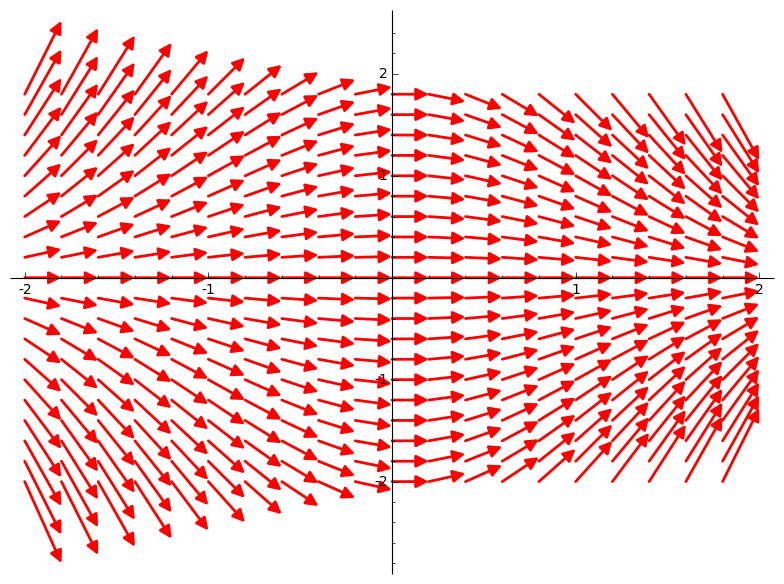
\includegraphics[scale=0.35]{figures/equadiff-courbe1.png} \qquad
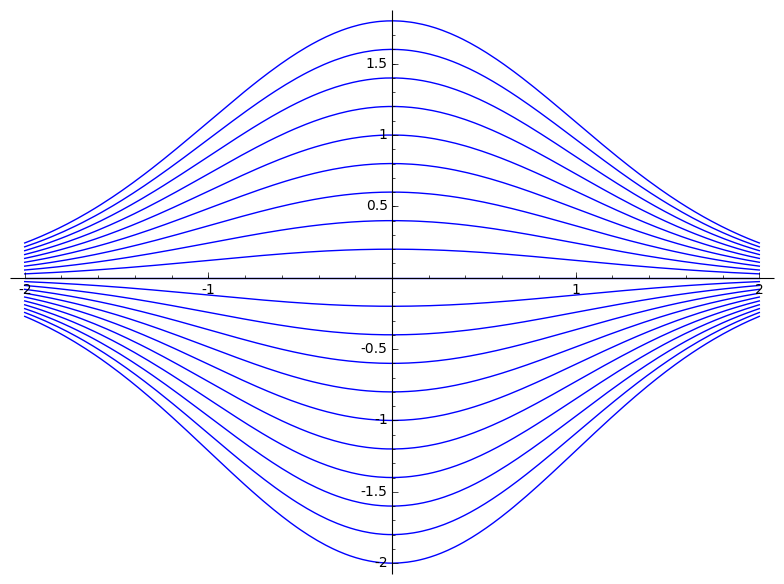
\includegraphics[scale=0.35]{figures/equadiff-courbe2.png} \\
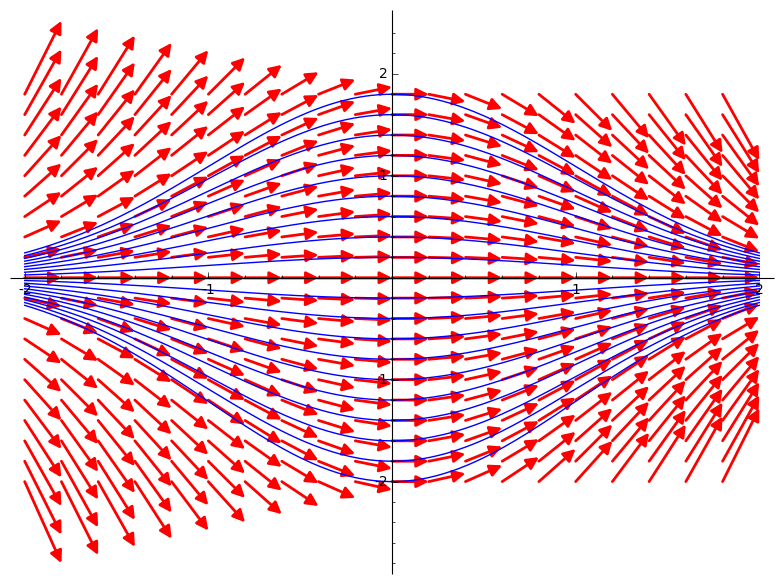
\includegraphics[scale=0.35]{figures/equadiff-courbe3.png} \qquad
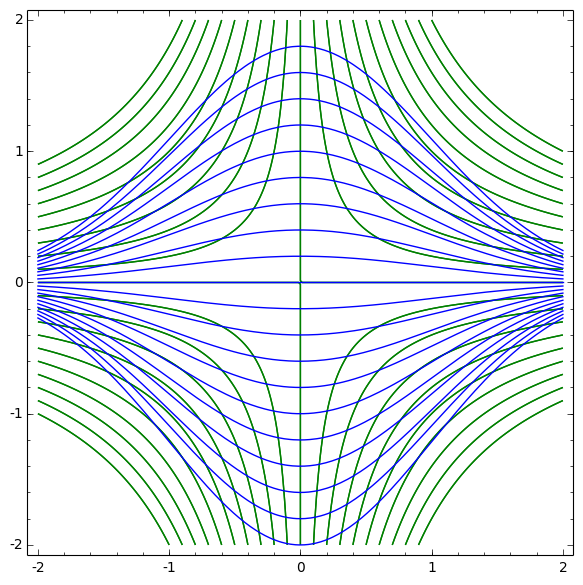
\includegraphics[scale=0.35]{figures/equadiff-courbe4.png} \\ 
\end{center}


\begin{enumerate}
  \item Voici comment tracer le champ de vecteurs associé à $y' = f(x,y)$.
  
  \insertcode{algos/equadiff-courbe-tex1.sage}{equadiff-courbe.sage (1)}
  
  \begin{itemize}
    \item Les variables de la fonction $f$ sont ici $u$ et $v$ pour ne pas interférer avec
  la variable $x$ et la fonction $y$.
  
    \item N'hésitez pas à renormaliser les vecteurs $v$, (par exemple en $v/10$) pour plus de lisibilité. 
  
    \item  En fait la fonction \codeinline{plot_vector_field}, prédéfinie dans \Sage, trace aussi les champs de
  vecteurs.
  \end{itemize}

  
 
 
  
  \item 
  \begin{enumerate}
    \item Les solutions de l'équation sont les
    $$y(x) = C \exp\left(-\frac{x^2}{2}\right) \quad \text{ où } \quad C \in \R.$$
    
    \item Le code suivant résout l'équation différentielle et trace la solution 
    avec la condition initiale $y(0)=k$, pour $k$ variant de \codeinline{kmin} à \codeinline{kmax}
    avec un pas de \codeinline{delta}.
    
\insertcode{algos/equadiff-courbe-tex2.sage}{equadiff-courbe.sage (2)}
    
    \item Les courbes intégrales forment une partition 
de l'espace : par un point il passe exactement une courbe intégrale. C'est 
une conséquence du théorème d'existence et d'unicité de Cauchy-Lipschitz. 
% Du point de vue de la physique, on pourrait dire que l'équation différentielle 
% régit le comportement d'un système qui évolue de manière déterministe.

  \end{enumerate}
  \item Les isoclines sont définies par l'équation $f(x,y) = c$.
  Elles se tracent par la commande \\
  \centerline{\codeinline{implicit_plot(f-c, (x,xmin,xmax), (y,ymin, ymax))}}
  
  Ici les isoclines ont pour équation $-xy=c$, ce sont donc des hyperboles.
  
\end{enumerate}



%--------------------------------------------------------
\subsection{\'Equations différentielles du second ordre}

\begin{tp}
L'équation différentielle
$$x''(t) +f x'(t)+ \frac{k}{m} x(t) = 0$$ 
correspond au mouvement d'une masse $m$ 
attachée à un ressort de constante $k>0$
et des frottements $f\ge0$.

  \myfigure{0.65}{
    \tikzinput{fig_formel_equadiff_ressort}\ \      
  }

Résoudre et tracer les solutions pour 
différentes valeurs de $f\ge0$ (prendre $k=1$, $m=1$), 
avec les conditions initiales :
$$x(0)= 1 \quad \text{ et } \quad x'(0)=0.$$
\end{tp}

Pour une valeur de $f$, l'équation se résout par : \\
\centerline{\codeinline{desolve(diff(x,t,2) + f*diff(x,t) + k/m*x(t) == 0, x, ics=[0,1,0])}}

Voici les solutions pour $f=0$, $f=1$ et $f=2$ :

\begin{center}
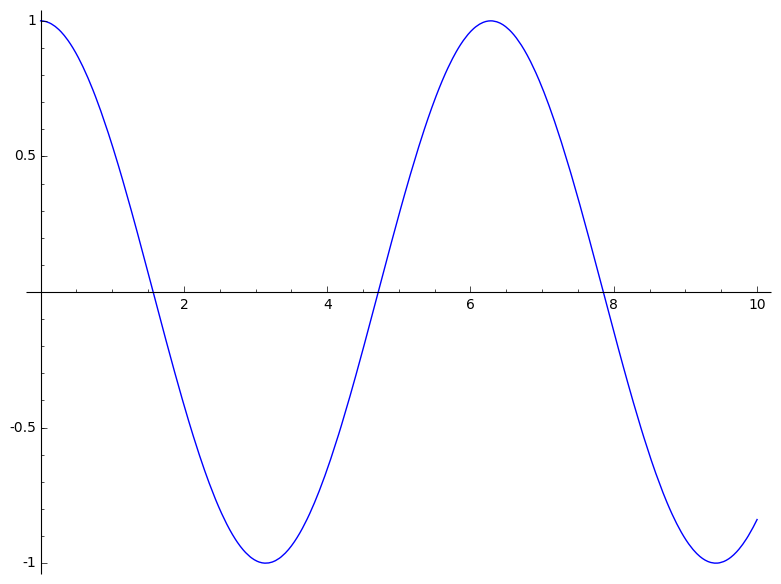
\includegraphics[scale=0.25]{figures/equadiff-ressort1} \quad
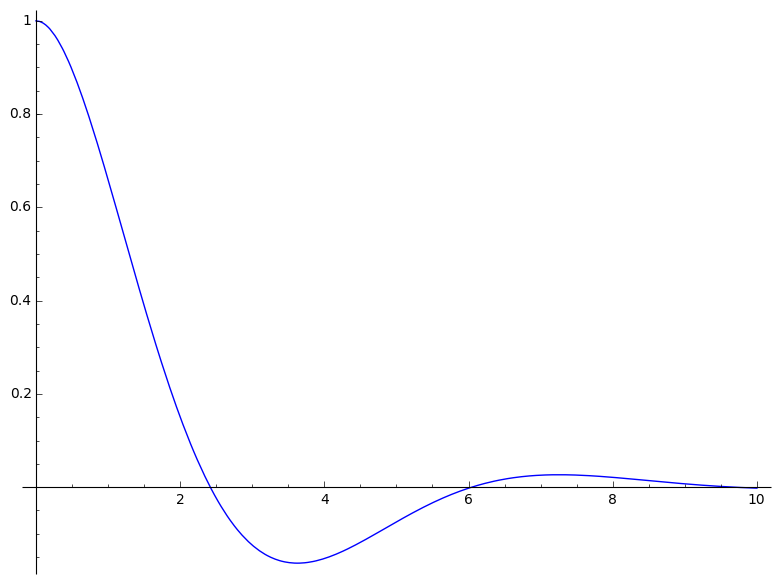
\includegraphics[scale=0.25]{figures/equadiff-ressort2} \quad
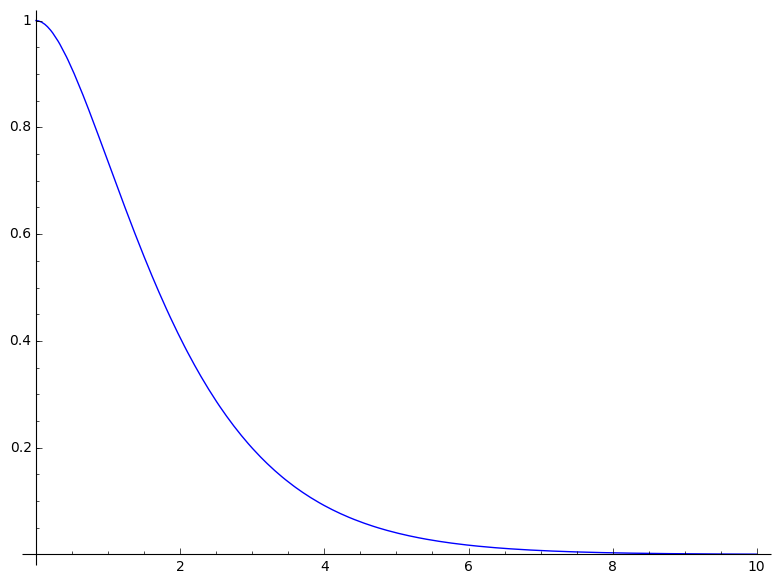
\includegraphics[scale=0.25]{figures/equadiff-ressort3} 
\end{center}


\begin{itemize}
  \item Cas $f=0$. Il n'y a pas de frottement. L'équation différentielle s'écrit
  $x''+ \frac{k}{m} x = 0$. Pour $k=1$, $m=1$ alors l'équation est simplement 
  $x''+ x = 0$ dont les solutions sont de la forme
  $$x(t) = \lambda \cos t + \mu \sin t \qquad \lambda,\mu \in\Rr.$$
  Avec les conditions initiales $x(0)=1$ et $x'(0)=0$, l'unique solution est 
  $$x(t) = \cos t.$$
  Il s'agit donc d'un mouvement périodique.
  
  \item Cas $0 < f < 2$. Les frottements sont faibles.
  Par exemple pour $f=1$ la solution est 
  $$\left(\frac{\sqrt{3}}{3} \sin\left(\frac{\sqrt{3}}{2} t\right) + 
   \cos\left(\frac{\sqrt{3}}{2} t\right)\right)
  e^{-\frac{1}{2} t}. $$
  Il s'agit d'un mouvement amorti oscillant autour de la position d'origine $x=0$.
  
  \item Cas $f \ge 2$. Les frottements sont forts. 
  Par exemple pour $f=2$ la solution est
  $$x(t) = (t + 1)e^{-t}.$$
  Il n'y a plus d'oscillations autour de la position d'origine.
\end{itemize}


\finchapitre

\end{document}

